% This text is proprietary.
% It's a part of presentation made by myself.
% It may not used commercial.
% The noncommercial use such as private and study is free
% May 2007
% Author: Sascha Frank 
% University Freiburg 
% www.informatik.uni-freiburg.de/~frank/
%
% 
\documentclass{beamer}
\setbeamertemplate{navigation symbols}{}

\usepackage{beamerthemeshadow}


% JW: packages:
\usepackage{amsmath}
\usepackage{graphicx}
\usepackage{fontawesome}
\usepackage{dashrule}
% \usepackage[my options...]{xcolor}:
% NOTE: xcolor is already loaded by beamer.
% When it's loaded with options, compilation will fail.
% If needed, instead before documentclass{beamer} write this:
% PassOptionsToPackage{my options...}{color}.
\usepackage{hyperref}
\hypersetup{
    colorlinks,
    linkcolor={red!50!black},
    citecolor={blue!50!black},
    urlcolor={blue!80!black}
}

% JW: beamer config (can be changed locally)
\setbeamercovered{transparent} % show items in unspecified slides as gray




\begin{document}
\title{SiScLab Project 8}  
\author{Katta, Partmann, Wasmer}
\date{\today} 

\begin{frame}
\titlepage
\end{frame}

% 
\chapter{Introduction}
\label{chap:intro}

\subsection{Problem Statement}
Solid State physics deals with the study of large scale properties of solid materials resulting from the atomic scale properties. A solid state physicist can get to know the atomic scale properties from the experiments conducted on the material. One such experiment is DFT(Density Functional theory). This method or experiment is computational Quantum mechanical modelling method to investigate the electronic structure of many body systems of an atom or molecule. Electron density, Inter molecular forces, charge transfer excitations, calculation of band gap are few extractions from DFT  simulations. 

Fleur is one such DFT simulation which is made by physicist at Juelich Forchungzentrum and most importantly its an open source and anyone can access it and use it. Like any other simulation, DFT simulation also outputs a lot of data so that a solid state physicist can understand and determine the properties of a cell structure of a molecule and from there any physical properties of the material can be determined thereafter. Fleur can be run by digitally specifying the cell structure of a molecule and so can be run to any material and such outputs.

Generally it is used to find/simulate properties of solids with impurities in cell structure. Fluer outputs the data of DFT simulation. It gives the data of ground state and excited state properties of solids. These data which are raw are generally not accessible directly and have to be processed through steps for the solid state physicist to understand the raw data extracted from Fleur DFT simulation. This becomes the major problem and which is dealt in this project. The goal of this project was to implement a complete data analysis pipeline for this application. The steps include preprocessing followed by data exploration and visualization.

\subsection{Motivation and Requirements}

An API which solves the physicist's problem of understanding the simulation data which transforms raw data to useful data such that it is process and visualizes. This API has to process the output files from fleur directly so that it is easier for physicists to get the data processed without external effort. Having said this, modularization and easy maintainability of code also matters since the simulation output keeps varying over the time with the development of simulation code and more data getting collected from simulation.

This API shouldn't only be solving the physicist's problem but also should be fast enough in terms of computation. As known, using of computer code to get outputs and may cause confusions. So an front end GUI is needed such that a physicist can use the GUI to output the processed data. As this is used for research purpose and the features such as plots, images and other should be of high quality so that there is no uncertainty of the results.

\subsection{Steps}

As a project, step by step procedure has completed to complete the task of processing and visualization.
\begin{itemize}
\item Understanding the problem: Firstly the theory of DFT simulation, Fleur code, band plots, density plots, file format of data and other necessary theory needed are learnt and understanding about the problem.
\item Pre Processing: Once problem is clearly understood, first step of project comes to preprocessing the data. Reading the data, sorting the data and storing it sorted which can be used in further stages of implementation.
\item Exploring the data: From the raw data, not just band plots but many features can be extracted from the raw simulation data. Finding out through exploring the data and trying to understand and extract those features.
\item Visualization: The data which is preprocesed and extracted need to be visualized into plots such that any user with solid state physics background can understand it by a glance.
\item Front End: A GUI is developed so that its easier in future for any physicist to just run the GUI and get the plots instead of going through whole code.
\item Results and lookup: Getting to know the features extracted, studying it, reporting the same.

\end{itemize}
%%% Local Variables:
%%% mode: latex
%%% TeX-master: "../"
%%% End:

% 
\chapter{Theoretical Background}
\label{chap:theory}

...some introduction scentence depending on into chapter...

%The visualization pipeline developed in this project is supposed to process data that is produced by the scientific code Fleur \cite{fleur}.

Fleur computes the electronic structure in crystals using the Density Functional Theory approach (DFT), which is the state of the art method for this problem. The many-body Schrödinger equation, that can be used to describe electrons in solids, is almost impossible to solve directly, because the storage of the wavefunctions of each of the $N$ electrons in the system at each spatial coordinate exceeds the available memory of any currently available computer for even quite small $N$. This motivates the DFT approach, that uses two fundamental theorems to reduce the computational complexity of the many-body problem significantly. The Hohenberg-Kohn theorem allows to use the electron density instead of the $N$-electron wavefunctions to uniquely characterize the ground state of a system. With the Kohn-Sham equations, the interacting Hamiltonian of the system can be replaced by non-interacting equations with an effective potential. This approach reduces the dimensionality of the problem from $N^3$ to $3$ and trades the interacting Hamiltonian for a set of non-interacting equations that have to be solved self-consistently. In general, the DFT approach is not just limited to computations of electrons in crystals, but is also for example used in chemestry to compute nonperiodic molecules.
% 
The output of a DFT calculation includes various physical quantities (for example the 3-dimensional spatial electron density, which is the central quantity in DFT calculations), but for this project we focus on two quantities that are easy to interpret, already reduced in dimensionality and frequently used in both experimental and theoretical physics.

The band structure $E(\vec{k})$ represents the eigenenergies of the eigenfunctions of the Hamiltonian for each crystal momentum $\vec{k}$. It represents the dispersion relation of electrons in the crystal and relates allowed momenta and energies. In general, $E(\vec{k})$ is defined at any point inside the Brillouin zone, which is a special choice of the unit cell in the reciprocal lattice of the crystal. Both, the real-space lattice and the reciprocal lattice are shown for a face centered cubic (fcc) crystal in figure \textbf{TODO}. For larger unit cells with fewer symmetries, the Brillouin zone can be much more complicated than in the shown example. In order to reduce the dimensionality of $E(\vec{k})$ with $k \in {\rm I\!R}^3$, the dispersion relation is only sampled along a discrete one-dimensional path between high symmetry points in the Brillouin zone. This path still contains most of the relevant physical features.

The second central quantity in this project is the Density of States (DOS) $D(E)$, which describes the number of states per energy interval, which is independent from its corresponding crystal momentum. In this sense, the DOS is also derived from $E(\vec{k})$, but instead of just selecting a subset, the $\vec{k}$ dependency is summed out. Both complementary quantities together are a common choice for comprehensively visualizing electronic structure data while still capturing most of the important physics. 

For applications, it is useful to investigate where the contributions to $E(k)$ and $D(E)$ come from. Therefore, the data contains the weights of each basis function of the DFT calculation belonging to the individual atom groups and the orbitals. This means, spatial information about the system can be restored by considering only contributions from certain atom groups. (An atom group contains all atoms that are equivalent with respect to symmetries of the real space lattice.) On the other hand, the projection on the hydrogen orbitals s, p, d, f encode information about the shape of the wavefunction at each atom. These contributions are stored in the form of relative weights that can be summed to include contributions for multiple groups and orbitals. In case of distinct spins in the crystal, $E(k)$, $D(E)$ and the weights can be different for both spins and are therefore stored individually.



%%% Local Variables:
%%% mode: latex
%%% TeX-master: "../report"
%%% End:

%% It is just an empty TeX file.
%% Write your code here.

\section{Implementation}
\label{sec:implementation}
% logo definitions
\newcommand{\logoFleur}{%
  \begingroup\normalfont
  \includegraphics[height=1.2\fontcharht\font`\B]{img/logo/fleur.png}%
  \endgroup
}
\newcommand{\logoAiida}{%
  \begingroup\normalfont
  \includegraphics[height=1.0\fontcharht\font`\B]{img/logo/aiida.png}%
  \endgroup
}
\newcommand{\logoAiidalab}{%
  \begingroup\normalfont
  \includegraphics[height=1.0\fontcharht\font`\B]{img/logo/aiidalab.png}%
  \endgroup
}
\newcommand{\logoBinder}{%
  \begingroup\normalfont
  \includegraphics[height=1.2\fontcharht\font`\B]{img/logo/binder.png}%
  \endgroup
}
\newcommand{\logoBokeh}{%
  \begingroup\normalfont
  \includegraphics[height=1.2\fontcharht\font`\B]{img/logo/bokeh.png}%
  \endgroup
}
\newcommand{\logoDash}{%
  \begingroup\normalfont
  \includegraphics[height=1.2\fontcharht\font`\B]{img/logo/dash.png}%
  \endgroup
}
\newcommand{\logoDocker}{%
  \begingroup\normalfont
  \includegraphics[height=1.2\fontcharht\font`\B]{img/logo/docker.png}%
  \endgroup
}
\newcommand{\logoHoloviews}{%
  \begingroup\normalfont
  \includegraphics[height=1.2\fontcharht\font`\B]{img/logo/holoviews.png}%
  \endgroup
}
\newcommand{\logoHvplot}{%
  \begingroup\normalfont
  \includegraphics[height=1.2\fontcharht\font`\B]{img/logo/hvplot.png}%
  \endgroup
}
\newcommand{\logoJavascript}{%
  \begingroup\normalfont
  \includegraphics[height=1.2\fontcharht\font`\B]{img/logo/javascript.png}%
  \endgroup
}
\newcommand{\logoJupyter}{%
  \begingroup\normalfont
  \includegraphics[height=1.2\fontcharht\font`\B]{img/logo/jupyter.png}%
  \endgroup
}
\newcommand{\logoMatplotlib}{%
  \begingroup\normalfont
  \includegraphics[height=1.2\fontcharht\font`\B]{img/logo/matplotlib.png}%
  \endgroup
}
% \newcommand{\logoMpld3}{%
%   \begingroup\normalfont
%   \includegraphics[height=1.2\fontcharht\font`\B]{img/logo/mpld3.png}%
%   \endgroup
% }
\newcommand{\logoPanel}{%
  \begingroup\normalfont
  \includegraphics[height=1.2\fontcharht\font`\B]{img/logo/panel.png}%
  \endgroup
}
\newcommand{\logoParam}{%
  \begingroup\normalfont
  \includegraphics[height=1.2\fontcharht\font`\B]{img/logo/param.png}%
  \endgroup
}
\newcommand{\logoPlotly}{%
  \begingroup\normalfont
  \includegraphics[height=1.2\fontcharht\font`\B]{img/logo/plotly.png}%
  \endgroup
}
\newcommand{\logoPython}{%
  \begingroup\normalfont
  \includegraphics[height=1.2\fontcharht\font`\B]{img/logo/python.png}%
  \endgroup
}
\newcommand{\logoPyviz}{%
  \begingroup\normalfont
  \includegraphics[height=1.2\fontcharht\font`\B]{img/logo/pyviz.png}%
  \endgroup
}
\newcommand{\logoSeaborn}{%
  \begingroup\normalfont
  \includegraphics[height=1.2\fontcharht\font`\B]{img/logo/seaborn.png}%
  \endgroup
}

%%% Local Variables:
%%% mode: latex
%%% TeX-master: t
%%% End:


\newcommand{\theimage}{\includegraphics[width=0.8\linewidth]{img/module_design.png}}% Shorthand
\begin{frame}\frametitle{Module Design Goals}
    \begin{columns}
        \begin{column}{.4\textwidth}
            \centerline{\theimage}
        \end{column}
        \begin{column}{.6\textwidth}
            \visible<1->{Multifunctionality:
            \begin{itemize}            
            \item automated workflows like in \logoAiida{}
            \item manual data analysis with Python
            \end{itemize}}
            \visible<2->{\hdashrule{\textwidth}{1pt}{1pt}
            \begin{itemize}
            \item no boilerplate code!
            % \vspace{0.5em}
            \end{itemize}}
            \visible<3->{\hdashrule{\textwidth}{1pt}{1pt}
            \begin{itemize}
            \item Desktop \faDesktop{}
            \item Web \faServer{} \faArrowRight{} \faGlobe{} like in \logoAiidalab{}
            \end{itemize}}
        \end{column}
    \end{columns}
\end{frame}
% Talking Notes:
% TODO

\subsection{Preprocessor}
\label{sec:preprocessor}

\renewcommand{\theimage}{\includegraphics[width=1.2\linewidth]{img/reader_flowchart4.png}}% Shorthand
\begin{frame}\frametitle{Preprocessor Module}
    \begin{columns}
        \begin{column}{.55\textwidth}
            \visible<3->{\centerline{\theimage}}            
        \end{column}

        \begin{column}{.4\textwidth}
            \visible<1->{Input: Fleur calculation results stored in Hierarchical Data Format
            (HDF).}
            \visible<2->{Combining \emph{Python AB\(C^1\) and \emph{type
                  introspection}} enables concise \textbf{Recipes} for different applications:}
            \begin{itemize}
            \item<4-> \faArrowRight{} attribute dependency resolution
            \item<5-> \faArrowRight{} modular output types
            \end{itemize}
        \visible<2->{\textsuperscript{1}Abstract Base Class}            
        \end{column}
    \end{columns}
\end{frame}
% Talking Notes:
% - HDF: like a file system with metadata annotation
% - Recipe: build class at runtime (introspection), with transformed attributes (HDF datasets) and
%   application-specific functions, and instantiate object.
% - Dependency resolution: user does not have to take care of order in which
%   arguments are processed (alphabetic ordering)
% - Transforms Dependency example: coordinate transformation
% - Reusability: new recipes may be composed for different workflows with minimal effort
% - Abstract base classes define general and specific Transforms and Output Types
% - Output type example: FleurBands

\begin{frame}\frametitle{Data Selection for Visualization}    
    Application Band Structure Viz.: from 4D discrete weighted points to 2D bands.
    \begin{align*}
      W^{\text{eff}}_{s,k,\nu} = \left( \frac{\sum\limits_{\substack{g \in \text{groups} \\ l \in \text{characters}}} n_{s,k,\nu,g,l} N_g}{\sum\limits_{\substack{g \in \text{all groups} \\ l \in \text{all characters}}} n_{s,k,\nu,g,l} N_g} \right) \left(W_{s,k,\nu}^{\text{unf}}\right)^\alpha
    \end{align*}
    \vspace{1em}
    \begin{itemize}
    \item<2-> \(W^{\text{eff}}_{s,k,\nu}\): effective weight
    \item<3-> \(s\) spin, \(k\) point on \(k\)-path, \(\nu\) band, \(g\)
        group, \(l\) character
    \item<4-> \(n_{s,k,\nu,g,l}\): State-specific \(l\)-like charge
    \item<5-> \(N_g\): no. of atoms in group         
    \item<6-> \(W_{s,k,\nu}^{\text{unf}}\): unfolding weight; \(\alpha =0\implies \) no unfolding
    \end{itemize}

    
\end{frame}
% Slide notes:
% - Reference: Bluegel FLAPW https://www.fz-juelich.de/SharedDocs/Downloads/PGI/PGI-1/DE/SB_NIC_pdf.pdf?__blob=publicationFile
% - indices: nu = band index, mu = muffin tin (i.e. atom, probably corresponds
% to atom group index), l = angular
% quantum number?
% - s = spin, k = k vector, g atom group, G_g atoms_per_group
% - alpha = unfolding weight exponent
% 
% Talking Notes:
% - get_data method

\begin{frame}
    \frametitle{Data Selection for Viz}
    % ballpark calculation: spins 2, k 500, bands 400, groups 20, chars 4
    Typically, \(\sim 10^7\) data points are accessed.
    \pause
    \vspace{2em}
     
    Optimizations:
    \pause
    \begin{itemize}
    \item reshaping \((k,\nu) \rightarrow (k \cdot \nu)\)
        \pause
    \item weight filter \(t\): \(W^{\text{eff}}_{s,k,\nu} > t\)
        \pause
    \item using optimized \texttt{numpy} functions for tensor product
        \pause
    \item buffering on selection change
    \end{itemize}
    \pause 
    \faArrowRight{} Speedup \(\sim 10^2\)
\end{frame}

\subsection{Interactive Visualization}
\label{sec:visualization}

\renewcommand{\theimage}{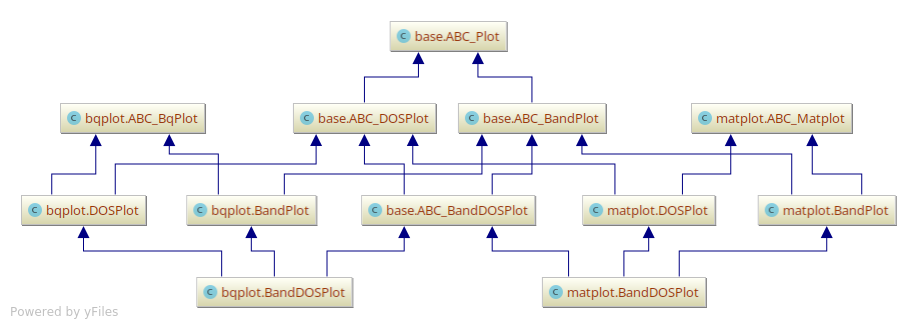
\includegraphics[width=1.1\linewidth]{img/pycharm_uml/matplot.png}}% Shorthand
\begin{frame}\frametitle{Visualization Module}
    \begin{itemize}
    \item<1-> Combine \emph{Python ABC} and \emph{multiple inheritance}
    \item<2-> \faArrowRight{} maximizes code reuse for different applications
        and viz. libraries employed
    \end{itemize}    
    \visible<3->{\centerline{\theimage}}
\end{frame}

\subsection{Desktop Frontend}
\label{sec:desktop-frontend}

\begin{frame}\frametitle{Desktop Frontend}
    Choice of GUI Toolkit: \textbf{TKinter} over (Kivy, PySide/PyQt, ...)

    Choice of Plotting tool: \textbf{matplotlib}
\end{frame}

\subsection{Web Frontend}
\label{sec:web-frontend}

\renewcommand{\theimage}{\includegraphics[width=1.0\linewidth]{img/py-viz-landscape.png}}% Shorthand
\begin{frame}\frametitle{Web Frontend}
    \visible<1->{The Python Visualization Landscape as of 2017...}
    \visible<2->{
      \centerline{\theimage}
      \begin{tiny}
          \href{https://github.com/rougier/python-visualization-landscape}{Python
            Visualization Landscape} by \href{https://github.com/rougier}{rougier} / BSD-2    
      \end{tiny}} 
\end{frame}

\begin{frame}\frametitle{Web Frontend}
    \begin{itemize}
    \item<1->Needed: a \textbf{survey} of OSS Frameworks for building a Web
        Dashboard using \textbf{only} \logoPython{}.
    \item<2-> Selection Process: \emph{Framework supports...}
        \begin{itemize}
        \item<3-> I. \emph{... interactive graphical control
              elements ('widgets') to control plots}
        \item<4-> II. \emph{... easy deployment}
        \item<5-> III. \emph{... some actual plotting libraries}
        \end{itemize}        
    \end{itemize}
\end{frame}

\begin{frame}\frametitle{Web Frontend}
    \begin{table}
        \resizebox{\textwidth}{!}{%
          \begin{tabular}{c||c|c|c|c}
            \visible<1->{I. \textbf{Widgets} & \logoJupyter{} jupyter & pyviz \logoPanel{} panel & \logoBokeh{} bokeh & \logoDash{} dash \\\hline
            Languages & \logoPython{} & \logoPython{} & \logoPython{} / \logoJavascript{} & \logoPython{} / \logoJavascript{} \\\hline}
            \visible<2->{II. \textbf{Deployment} & & & & \\
            - Jupyter & \faCheck{} & \faCheck{} & \faCheck{} & \faCheck{} \\
            - Standalone\footnote{Excluded: writing from scratch using Flask} & (\logoBinder{}, \logoDocker{})\footnote{workaround. See also: \href{https://github.com/oschuett/appmode}{appmode}, \href{https://github.com/QuantStack/voila}{voila}, \href{https://github.com/minrk/thebelab}{thebelab}} & \logoBokeh{} server & \logoBokeh{} server & \logoPlotly{} plotly \\\hline}
            \visible<3->{III. \textbf{Plots}\footnote{interactive only}  & & & & \\
            - 2D & \logoMatplotlib{} mpl, bqplot, \textbf{all}  \faArrowLeft{} & \logoHvplot{} hvplot,  \faArrowRight{} \textbf{most} \faArrowLeft{}  & \logoBokeh{} & \logoPlotly{}\\
            - 3D & ipyvolume, \textbf{all}  \faArrowLeft{} & \faClose{} & \logoBokeh{} & \logoPlotly{}}
          \end{tabular}
        }
    \end{table}
\end{frame}
% Talking Notes:
% - Our decision:
%   - PyViz best (abstract GUI declaration supports Tkinter) but no 3D for atom plots, so out again
%   - Jupyter > (Bokeh, Dash) but expect deployment in AiiDAlab (JupyterHub) so simpler
%   - problem: standalone will now be harder, but maybe possible through binder
%   - 2D: matplotlib first cause same as Tkinter, for now
%   
 







% 


%% It is just an empty TeX file.
%% Write your code here.

\section{Applications} 

\begin{frame}\frametitle{Effective mass and Fermi velocity:}
\begin{itemize}

\item Derived Quantities:


    \item mass, that an electon in a crystal appears to have compared to a free electron (due to interactions in the solid)
    \item $m^{*} = \hbar^2  \frac{d^2E(k)}{dk^2}$
    \
    \item Group velocity at the Fermi energy
    \item $v_{Fermi} = \frac{dE(k)}{dk}$ at $E = E_F$ 


    \item Bandstructure periodic: Using FFT to compute accurate Derivates:
    \item $\Leftrightarrow$ Differentiate finite Fourier Series
    $f^{(n)}(x) = \mathcal{F}^{-1}\left((ik)^n\mathcal{F}(f(x))\right)$
\end{itemize}
\end{frame}
%% It is just an empty TeX file.
%% Write your code here.

\section{Conclusion} 

\begin{frame}
\frametitle{Conclusion}
\begin{itemize}
     \item<1-> Developed a package to visualize DFT data in a physically correct way
     \item<2-> Easy to use API and graphical interface
     \item<3-> studied data to extract pyhsical features ($m^*$, $v_{fermi}$) using
         numerical differentiation techniques
     \item<4-> Useful in physics research:
     \begin{itemize}
         \item<5-> Make Fleur output easily accessible to non-experts
         \item<6-> facilitate output \faArrowRight{} input conversion to other
             simulation codes while HDF format develops
         \visible<7->{\item possible to integrate into \logoAiida{} workflow}
         \item<8-> create small apps to calculate certain physical properties 
     \end{itemize}
\end{itemize}
\end{frame}



\end{document}
%%% Local Variables:
%%% mode: latex
%%% TeX-master: t
%%% End:
